%%%%%%%%%%%%  Generated using docx2latex.com  %%%%%%%%%%%%%%

%%%%%%%%%%%%  v2.0.0-beta  %%%%%%%%%%%%%%

\documentclass[12pt]{article}
\usepackage{amsmath}
\usepackage{latexsym}
\usepackage{amsfonts}
\usepackage[normalem]{ulem}
\usepackage{array}
\usepackage{amssymb}
\usepackage{graphicx}
\usepackage[backend=biber,
style=numeric,
sorting=none,
isbn=false,
doi=false,
url=false,
]{biblatex}\addbibresource{bibliography.bib}

\usepackage{subfig}
\usepackage{wrapfig}
\usepackage{wasysym}
\usepackage{enumitem}
\usepackage{adjustbox}
\usepackage{ragged2e}
\usepackage[svgnames,table]{xcolor}
\usepackage{tikz}
\usepackage{longtable}
\usepackage{changepage}
\usepackage{setspace}
\usepackage{hhline}
\usepackage{multicol}
\usepackage{tabto}
\usepackage{float}
\usepackage{multirow}
\usepackage{makecell}
\usepackage{fancyhdr}
\usepackage[toc,page]{appendix}
\usepackage[hidelinks]{hyperref}
\usetikzlibrary{shapes.symbols,shapes.geometric,shadows,arrows.meta}
\tikzset{>={Latex[width=1.5mm,length=2mm]}}
\usepackage{flowchart}\usepackage[paperheight=11.69in,paperwidth=8.27in,left=0.98in,right=0.98in,top=0.98in,bottom=0.98in,headheight=1in]{geometry}
\usepackage[utf8]{inputenc}
\usepackage[T1]{fontenc}
\TabPositions{0.49in,0.98in,1.47in,1.96in,2.45in,2.94in,3.43in,3.92in,4.41in,4.9in,5.39in,5.88in,}

\urlstyle{same}


 %%%%%%%%%%%%  Set Depths for Sections  %%%%%%%%%%%%%%

% 1) Section
% 1.1) SubSection
% 1.1.1) SubSubSection
% 1.1.1.1) Paragraph
% 1.1.1.1.1) Subparagraph


\setcounter{tocdepth}{5}
\setcounter{secnumdepth}{5}


 %%%%%%%%%%%%  Set Depths for Nested Lists created by \begin{enumerate}  %%%%%%%%%%%%%%


\setlistdepth{9}
\renewlist{enumerate}{enumerate}{9}
		\setlist[enumerate,1]{label=\arabic*)}
		\setlist[enumerate,2]{label=\alph*)}
		\setlist[enumerate,3]{label=(\roman*)}
		\setlist[enumerate,4]{label=(\arabic*)}
		\setlist[enumerate,5]{label=(\Alph*)}
		\setlist[enumerate,6]{label=(\Roman*)}
		\setlist[enumerate,7]{label=\arabic*}
		\setlist[enumerate,8]{label=\alph*}
		\setlist[enumerate,9]{label=\roman*}

\renewlist{itemize}{itemize}{9}
		\setlist[itemize]{label=$\cdot$}
		\setlist[itemize,1]{label=\textbullet}
		\setlist[itemize,2]{label=$\circ$}
		\setlist[itemize,3]{label=$\ast$}
		\setlist[itemize,4]{label=$\dagger$}
		\setlist[itemize,5]{label=$\triangleright$}
		\setlist[itemize,6]{label=$\bigstar$}
		\setlist[itemize,7]{label=$\blacklozenge$}
		\setlist[itemize,8]{label=$\prime$}



 %%%%%%%%%%%%  Header here  %%%%%%%%%%%%%%


\pagestyle{fancy}
\fancyhf{}
\chead{ 

%%%%%%%%%%%%%%%%%%%% Figure/Image No: 1 starts here %%%%%%%%%%%%%%%%%%%%


\begin{figure}[H]	\begin{subfigure}		\includegraphics[width=0.45\textwidth]{./../customXml/item1.xml}
	\end{subfigure}
~	\begin{subfigure}		\includegraphics[width=0.45\textwidth]{./numbering.xml}
	\end{subfigure}
~
\end{figure}


%%%%%%%%%%%%%%%%%%%% Figure/Image No: 1 Ends here %%%%%%%%%%%%%%%%%%%%


\vspace{\baselineskip}
}
\cfoot{ }
\renewcommand{\headrulewidth}{0pt}
\setlength{\topsep}{0pt}\setlength{\parskip}{8.04pt}
\setlength{\parindent}{0pt}

 %%%%%%%%%%%%  This sets linespacing (verticle gap between Lines) Default=1 %%%%%%%%%%%%%%


\renewcommand{\arraystretch}{1.3}


%%%%%%%%%%%%%%%%%%%% Document code starts here %%%%%%%%%%%%%%%%%%%%



\begin{document}

\vspace{\baselineskip}

\vspace{\baselineskip}
\begin{Center}
{\fontsize{28pt}{33.6pt}\selectfont \textbf{Langages et Environnements Évolués}\par}
\end{Center}\par

\begin{Center}
{\fontsize{24pt}{28.8pt}\selectfont \textbf{Choix d’options - AngularJs}\par}
\end{Center}\par


\vspace{\baselineskip}

\vspace{\baselineskip}


%%%%%%%%%%%%%%%%%%%% Figure/Image No: 2 starts here %%%%%%%%%%%%%%%%%%%%

\begin{figure}[H]
	\begin{Center}
		
\includegraphics[width=3.66in,height=3.68in]{./media/image1.jpeg}
	\end{Center}
\end{figure}


%%%%%%%%%%%%%%%%%%%% Figure/Image No: 2 Ends here %%%%%%%%%%%%%%%%%%%%

\par


\vspace{\baselineskip}

\vspace{\baselineskip}

\vspace{\baselineskip}

\vspace{\baselineskip}

\vspace{\baselineskip}

\vspace{\baselineskip}

\vspace{\baselineskip}
\textbf{Professeurs encadrants :\tab \tab \tab \tab }\tab \ \  \textbf{Réalisé par : }\par

Flavien BREUVART\tab \tab \tab \tab \tab  \ \  Magilan ELILTHAMILVALAVAN\par

Pierre BOUDES\tab \tab \tab \tab \tab \tab \ \  \par
\vspace{\baselineskip}
\vspace{\baselineskip}
\vspace{\baselineskip}
\vspace{\baselineskip}
\vspace{\baselineskip}
\vspace{\baselineskip}
\vspace{\baselineskip}
\vspace{\baselineskip}
\vspace{\baselineskip}
\vspace{\baselineskip}
\vspace{\baselineskip}
\vspace{\baselineskip}
\vspace{\baselineskip}
\vspace{\baselineskip}
\vspace{\baselineskip}
\vspace{\baselineskip}
\vspace{\baselineskip}
\vspace{\baselineskip}
\vspace{\baselineskip}
\vspace{\baselineskip}
\vspace{\baselineskip}
\vspace{\baselineskip}
\vspace{\baselineskip}

\section*{1) Description du projet}
\addcontentsline{toc}{section}{1) Description du projet}

\vspace{\baselineskip}
Le projet consiste à faire un site où les étudiants pourront entrer leurs choix d’options par classement de souhaits.\par

Cependant, les options ayant un effectif limité, il faut mettre en place un algorithme satisfaisant au mieux les souhaits des étudiants.\par

De plus, une partie administrateur pourra intervenir manuellement sur les affectations.\par


\vspace{\baselineskip}
\section*{2) Comment lancer le site}
\addcontentsline{toc}{section}{2) Comment lancer le site}

\vspace{\baselineskip}
Pour commencer vous devez installer Node.js (vous pourrez vérifier son installation en écrivant la commande « npm -v » et « node -v ») puis vous devez installer Angular CLI (vous pourrez vérifier son installation en écrivant la commande « ng -v »).\par

Allez sur https://github.com/magilan95/choisirlesoptions et téléchargez le dossier « choisirlesoptions » et dézippez le.\par

Vous trouverez les dossier choix et admin qui correspondent au projet Angular, le fichier cars2.sql qui vous permettra de créer les tables de la base de données « cars2 » que vous aurez à créer et vous trouverez aussi les dossier api et api2 que vous devrez placer dans votre serveur php (par exemple si c’est Wamp vous devrez le mettre dans le dossier www).\par

Après cela vous devez vous placer dans les dossiers « choix » et « admin » et lancer la commande « npm install –save » dans ces 2 fichiers.\par

Ensuite, vous pouvez lancer la page permettant aux élèves d’entrer leur choix en se positionnant dans le dossier « choix » puis lancer la commande « ng serve --o –port=4300 ».\par

De même vous pouvez lancer la page permettant aux administrateurs de modifié les choix d’options et de lancer l’algorithme qui place les élèves en se positionnant dans le dossier admin puis lancer la commande « ng serve --o ». \par


\vspace{\baselineskip}
\section*{3) Comment utiliser le site}
\addcontentsline{toc}{section}{3) Comment utiliser le site}

\vspace{\baselineskip}
\section{Site choix option}

\vspace{\baselineskip}
\begin{adjustwidth}{0.49in}{0.0in}
Lorsque l’étudiant arrive sur ce site il doit remplir le formulaire c’est-à-dire son numéro étudiant, sa moyenne (entre 0 et 20) et l’ordre dans lequel il souhaite choisir ses options.\par

\end{adjustwidth}



%%%%%%%%%%%%%%%%%%%% Figure/Image No: 3 starts here %%%%%%%%%%%%%%%%%%%%

\begin{figure}[H]
	\begin{Center}
		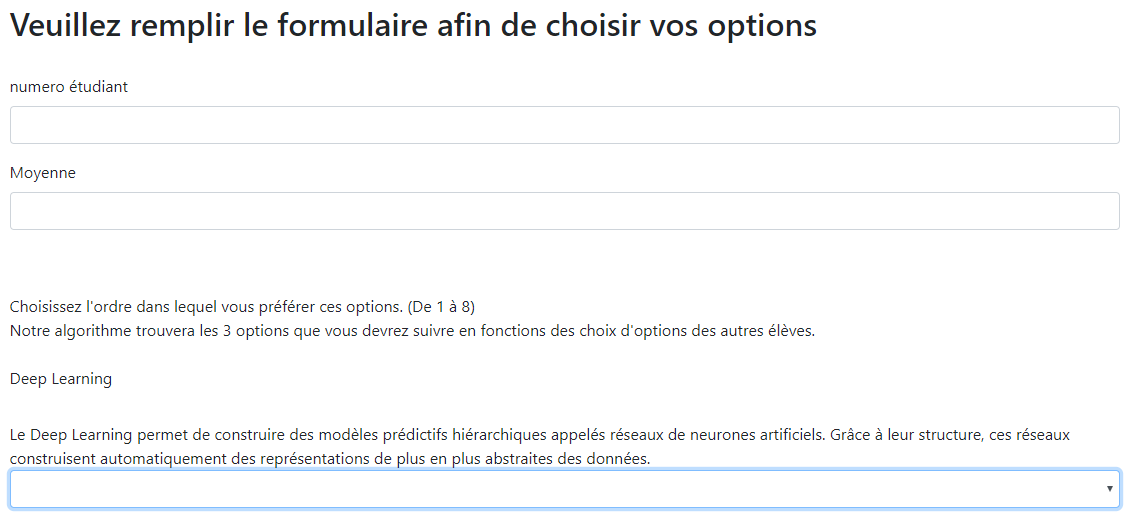
\includegraphics[width=6.29in,height=2.86in]{./media/image2.png}
	\end{Center}
\end{figure}


%%%%%%%%%%%%%%%%%%%% Figure/Image No: 3 Ends here %%%%%%%%%%%%%%%%%%%%

\par





\begin{adjustwidth}{0.49in}{0.0in}
Enfin il clique sur le bouton add afin d’ajouter son choix dans la base de données.\par
%%%%%%%%%%%%%%%%%%%% Figure/Image No: 4 starts here %%%%%%%%%%%%%%%%%%%%

\begin{figure}[H]
	\begin{Center}
		
\includegraphics[width=0.56in,height=0.42in]{./media/image3.png}
	\end{Center}
\end{figure}


%%%%%%%%%%%%%%%%%%%% Figure/Image No: 4 Ends here %%%%%%%%%%%%%%%%%%%%
\end{adjustwidth}

\begin{adjustwidth}{0.49in}{0.0in}
Le nombre d’élève dans la classe étant limité à 10, si les 10 étudiants ont entré leur choix il n’est plus possible de rentré d’autre choix à moins que l’administrateur supprime les choix d’un étudiant.\par

\end{adjustwidth}

\begin{adjustwidth}{0.49in}{0.0in}
En bas de la page se trouve un récapitulatif des choix des étudiants.\par

\end{adjustwidth}



%%%%%%%%%%%%%%%%%%%% Figure/Image No: 5 starts here %%%%%%%%%%%%%%%%%%%%

\begin{figure}[H]
	\begin{Center}
		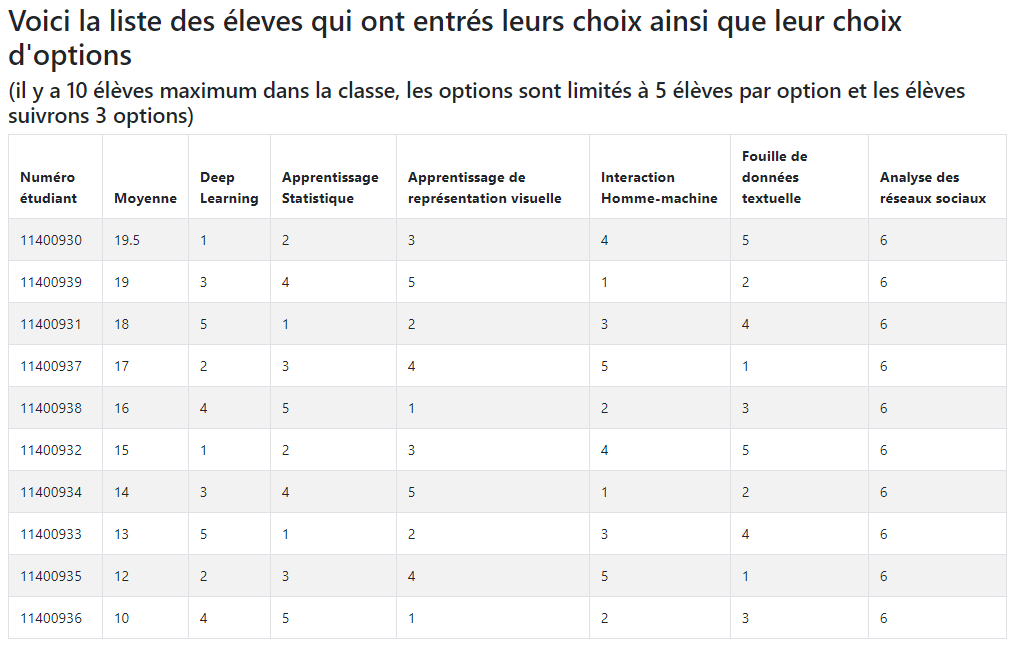
\includegraphics[width=6.3in,height=4.06in]{./media/image4.png}
	\end{Center}
\end{figure}


%%%%%%%%%%%%%%%%%%%% Figure/Image No: 5 Ends here %%%%%%%%%%%%%%%%%%%%

\par

\section{Site administrateur}

\vspace{\baselineskip}
\begin{adjustwidth}{0.49in}{0.0in}
Lorsque l’administrateur arrive sur le site administrateur, il a un aperçu de la liste des élèves qui ont entrés leurs choix qu’il peut modifier ou supprimer.\par

\end{adjustwidth}



%%%%%%%%%%%%%%%%%%%% Figure/Image No: 6 starts here %%%%%%%%%%%%%%%%%%%%

\begin{figure}[H]
	\begin{Center}
		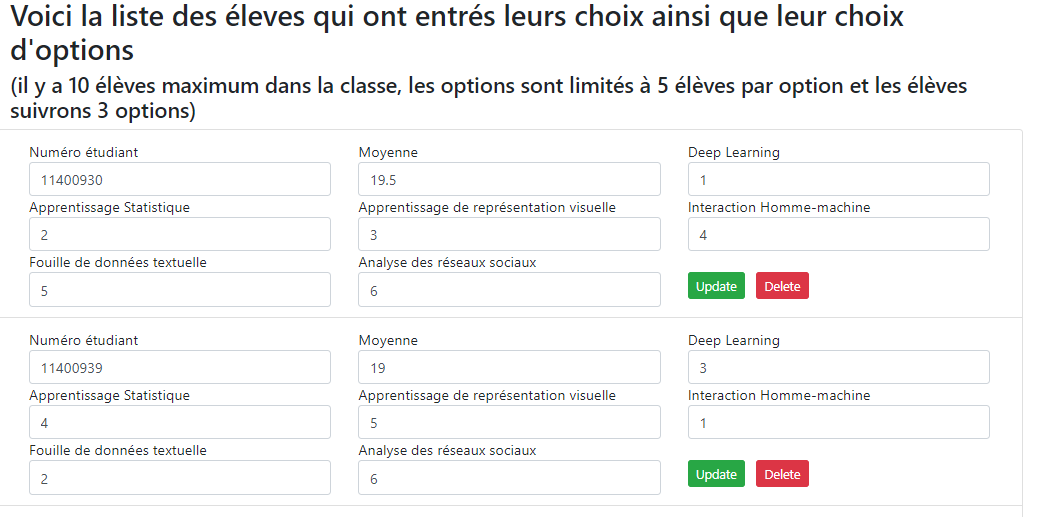
\includegraphics[width=6.3in,height=3.14in]{./media/image5.png}
	\end{Center}
\end{figure}


%%%%%%%%%%%%%%%%%%%% Figure/Image No: 6 Ends here %%%%%%%%%%%%%%%%%%%%

\par

\begin{adjustwidth}{0.49in}{0.0in}
Ensuite, juste en dessous ce trouve la liste des options ainsi que les élèves qui s’y trouvent. Cette liste peut être modifié par l’administrateur avec la seule règle que si l’ont veut ajouter un numéro étudiant il faut l’ajouter toujours dans l’ordre c’est-à-dire dans la case « premier élève » si c’est vide ou bien « deuxième » si la case « premier » est déjà prise etc$ \ldots $ \par

\end{adjustwidth}



%%%%%%%%%%%%%%%%%%%% Figure/Image No: 7 starts here %%%%%%%%%%%%%%%%%%%%

\begin{figure}[H]
	\begin{Center}
		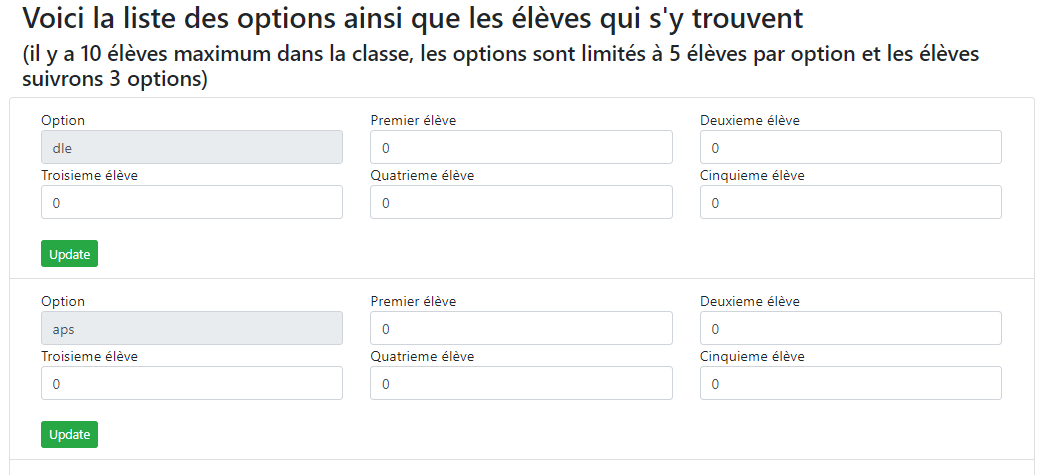
\includegraphics[width=6.3in,height=2.8in]{./media/image6.png}
	\end{Center}
\end{figure}


%%%%%%%%%%%%%%%%%%%% Figure/Image No: 7 Ends here %%%%%%%%%%%%%%%%%%%%

\par


\vspace{\baselineskip}

\vspace{\baselineskip}
\begin{adjustwidth}{0.49in}{0.0in}
Et enfin pour lancer l’algorithme il suffit de cliquer sur le bouton qui se trouve en dessous :\par

\end{adjustwidth}



%%%%%%%%%%%%%%%%%%%% Figure/Image No: 8 starts here %%%%%%%%%%%%%%%%%%%%

\begin{figure}[H]
	\begin{Center}
		
\includegraphics[width=6.29in,height=0.28in]{./media/image7.png}
	\end{Center}
\end{figure}


%%%%%%%%%%%%%%%%%%%% Figure/Image No: 8 Ends here %%%%%%%%%%%%%%%%%%%%

\par


\vspace{\baselineskip}
\tab Puis de rafraichir la page.\par

\begin{adjustwidth}{0.49in}{0.0in}
Ainsi pour voir les élèves après qu’ils soient ajoutés dans les options il suffit de regarder le tableau en fin de page.\par

\end{adjustwidth}



%%%%%%%%%%%%%%%%%%%% Figure/Image No: 9 starts here %%%%%%%%%%%%%%%%%%%%

\begin{figure}[H]
	\begin{Center}
		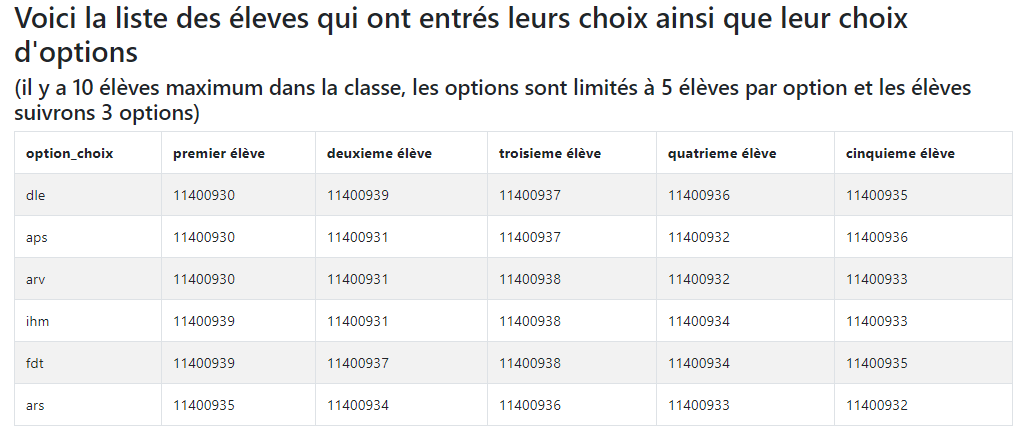
\includegraphics[width=6.29in,height=2.71in]{./media/image8.png}
	\end{Center}
\end{figure}


%%%%%%%%%%%%%%%%%%%% Figure/Image No: 9 Ends here %%%%%%%%%%%%%%%%%%%%

\par


\vspace{\baselineskip}

\printbibliography
\end{document}